\documentclass[14pt,a4paper]{scrartcl}
\usepackage[utf8]{inputenc}
\usepackage{ragged2e}
\usepackage{mathtools}
% \usepackage{esint}
\usepackage[english,russian, ukrainian]{babel}
\usepackage{misccorr,color,ragged2e,amsfonts,amsthm,graphicx,systeme,amsmath,mdframed,lipsum}
\renewcommand\qedsymbol{$\blacksquare$}
\renewcommand*{\proofname}{\text{Доведення}}
\theoremstyle{definition}
\newtheorem*{defo}{Означення}
\newtheorem*{teo}{Теорема}
\newtheorem*{example}{Приклад}
\theoremstyle{remark}
\newtheorem*{remark}{Зауваження}
\theoremstyle{definition}
\newtheorem*{consequence}{Наслідок}
\theoremstyle{definition}
\newtheorem{statement}{Утверждение}[section]
\newmdtheoremenv{boxteo}{Теорема}[section]
\setlength\parindent{0pt}
\DeclareMathOperator*\lowlim{\underline{lim}}
\DeclareMathOperator*\uplim{\overline{lim}}
\newcommand\independent{\protect\mathpalette{\protect\independenT}{\perp}}
\def\independenT#1#2{\mathrel{\rlap{$#1#2$}\mkern2mu{#1#2}}}

% Default fixed font does not support bold face
\DeclareFixedFont{\ttb}{T1}{txtt}{bx}{n}{12} % for bold
\DeclareFixedFont{\ttm}{T1}{txtt}{m}{n}{12}  % for normal

% Custom colors
\usepackage{color}
\definecolor{deepblue}{rgb}{0,0,0.5}
\definecolor{deepred}{rgb}{0.6,0,0}
\definecolor{deepgreen}{rgb}{0,0.5,0}

\usepackage{listings}

% Python style for highlighting
\newcommand\pythonstyle{\lstset{
language=Python,
basicstyle=\ttm,
otherkeywords={self},             % Add keywords here
keywordstyle=\ttb\color{deepblue},
emph={MyClass,__init__},          % Custom highlighting
emphstyle=\ttb\color{deepred},    % Custom highlighting style
stringstyle=\color{deepgreen},
frame=tb,                         % Any extra options here
showstringspaces=false            %
}}

\definecolor{javared}{rgb}{0.6,0,0} % for strings
\definecolor{javagreen}{rgb}{0.25,0.5,0.35} % comments
\definecolor{javapurple}{rgb}{0.5,0,0.35} % keywords
\definecolor{javadocblue}{rgb}{0.25,0.35,0.75} % javadoc

\lstset{language=C++,
basicstyle=\ttfamily,
keywordstyle=\color{javapurple}\bfseries,
stringstyle=\color{javared},
commentstyle=\color{javagreen},
morecomment=[s][\color{javadocblue}]{/**}{*/},
numbers=left,
numberstyle=\tiny\color{black},
stepnumber=2,
numbersep=10pt,
tabsize=4,
showspaces=false,
showstringspaces=false}


% Python environment
\lstnewenvironment{python}[1][]
{
\pythonstyle
\lstset{#1}
}
{}

% \begin{python}
%  c  o  d  e
%    .  .  .
% \end{python}

% Python for external files
\newcommand\pythonexternal[2][]{{
\pythonstyle
\lstinputlisting[#1]{#2}}}

% Python for inline
\newcommand\pythoninline[1]{{\pythonstyle\lstinline!#1!}}
%
% \begin{python}
% class MyClass(Yourclass):
%     def __init__(self, my, yours):
%         bla = '5 1 2 3 4'
%         print bla
% \end{python}

\begin{document}



\def\be{\begin{equation}}
\def\ee{\end{equation}}
% Definition
\def\bd{\begin{defo}}
\def\ed{\end{defo}}

% Box Theorem
\def\bbt{\begin{boxteo}}
\def\ebt{\end{boxteo}}

\def\i{\infty}

\def\d{\partial}

\begin{titlepage}

\begin{center}

\vspace*{0.1cm}
\vfill

{\huge \textbf{ТЕОРІЯ СТІЙКОСТІ}}\\
\vspace{5cm}
За лекціями Горбань Н.\\
\vspace{1cm}
Редактори: Терещенко Д.\\ \hspace{3.7cm} Людомирський Ю.

\vfill

2021

\end{center}
\end{titlepage}


\tableofcontents

\newpage

\section{Лекція 1}

Нормальні системи діф. рівнянь.

\be
\left\lbrace
\begin{gathered}
x'_1 (t) = f_1(t, x_1 (t), ... , x_n(t)) \\
x'_2 (t) = f_2(t, x_1 (t), ... , x_n(t)) \\
\vdots \\
    x'_n (t) = f_n(t, x_1 (t), ... , x_n(t)) \\
\end{gathered}\right.
\ee

\bd
 Системою диф. рівнянь n-го порядку в нормальній формі називається система вигляду(1), де $ f_i : D \to \mathbb{R}, D \subset \mathbb{R}^{n+1 }; i = \overline{1, n}$.\\
 Позначення:
$$ \overline{x} (t) = \begin{bmatrix}
 x_1(t) \\
 \vdots\\
 x_n(t)
\end{bmatrix} - \text{невідома вектор-функція}$$
$$
\overline{f} (t, \overline{x} (t)) = \begin{bmatrix}
 f_1 \\
 \vdots
 \\
 f_n
\end{bmatrix} \qquad \qquad D \to \mathbb{R}^{n}, D \subset \mathbb{R}^{n+1}
$$

Тоді (1): \fbox{ $  \overline{x}' (t) = \overline{f} (t, \overline{x} (t))$}
\ed

\def\rect{\textbf{П}}
\bd
\textbf{Розв'язком системи } (1) на $(\alpha , \beta)$ називається така вектор функція $\overline{x} (t) \in C(\alpha , \beta)$, що:\\
1. $(t, x_1 (t), ..., x_n(t))  \in D \quad \forall t \in (\alpha , \beta)$. \\
2. $ \overline{x} (t)$ перетворює (1) на тотожність на $(\alpha , \beta)$. \\
\textbf{Загальним розв'язком системи}  (1) називається n-параметрична сім'я розв'язків (1), що охоплює всі розв'язки системи.
\ed

Задача Коші. Для заданих $t_0, \overline{x}^{0} \in D$ знайти такий розв'язок (1), що $\overline{x} (t_0) = \overline{x}^{0}$.

Нехай $(t_0 , \overline{x}^0) \in D :  \textbf{П} = \left\lbrace (t, \overline{x}) \bigg |
 \left| t - t_0 \right| \leq a, \quad
 \left| \left| \overline{x} - \overline{x^{0}} \right|  \right| \leq  b;
 \right\rbrace $ .\\
 Розглядається задача Коші: $\begin{cases}
      \overline{x} ' (t)  =  \overline{f} (t, \overline{x}) \\
      \overline{x} (t_0) = \overline{x}^0
 \end{cases}$
\begin{boxteo}[Теорема Пеано]
$\overline{f} \in \mathbb{C} (\rect) \Longrightarrow $\\$  \Longrightarrow $існують розв'язки задачі Коші, принаймі на інтервалі: $$ I = (t_0 - h, t_0 + h); \quad h = \min{\left\lbrace a , \frac{b}{M}  \right\rbrace }, \quad M = \max_{\rect} \left| \left| \overline{f} (\overline{x}) \right|  \right| $$
\end{boxteo}
\begin{boxteo}[Теорема Пікара] Якщо виконуються умови:\\
    1) $f \in C (\rect)$ \\
    2) $ \exists L > 0 \quad \forall (t, \overline{x}^1 ), (t, \overline{x} ^2) \in \rect  :
    \left| \left| \overline{f} (t, \overline{x}^1) - \overline{f} (t, \overline{x}^2)  \right|   \right|  \leq  L \left|  \left| \overline{x_1} - \overline{x_2} \right|  \right| $
    Тоді, існує та єдиний розвязок задачі Коші, принаймі на інтервалі: $$ I = (t_0 - h, t_0 + h); \quad h = \min{\left\lbrace a , \frac{b}{M}  \right\rbrace }, \quad M = \max_{\rect} \left| \left| \overline{f} (\overline{x}) \right|  \right| $$
\end{boxteo}

\begin{boxteo}[про продовження]
    Нехай $\overline{f} \in \mathbb{C}(D), D \subset \mathbb{R}^{n+1}$ - деяка обмежена область. Нехай $(t_0, \overline{x}^0) \in D$ - задана точка.

    \begin{center} 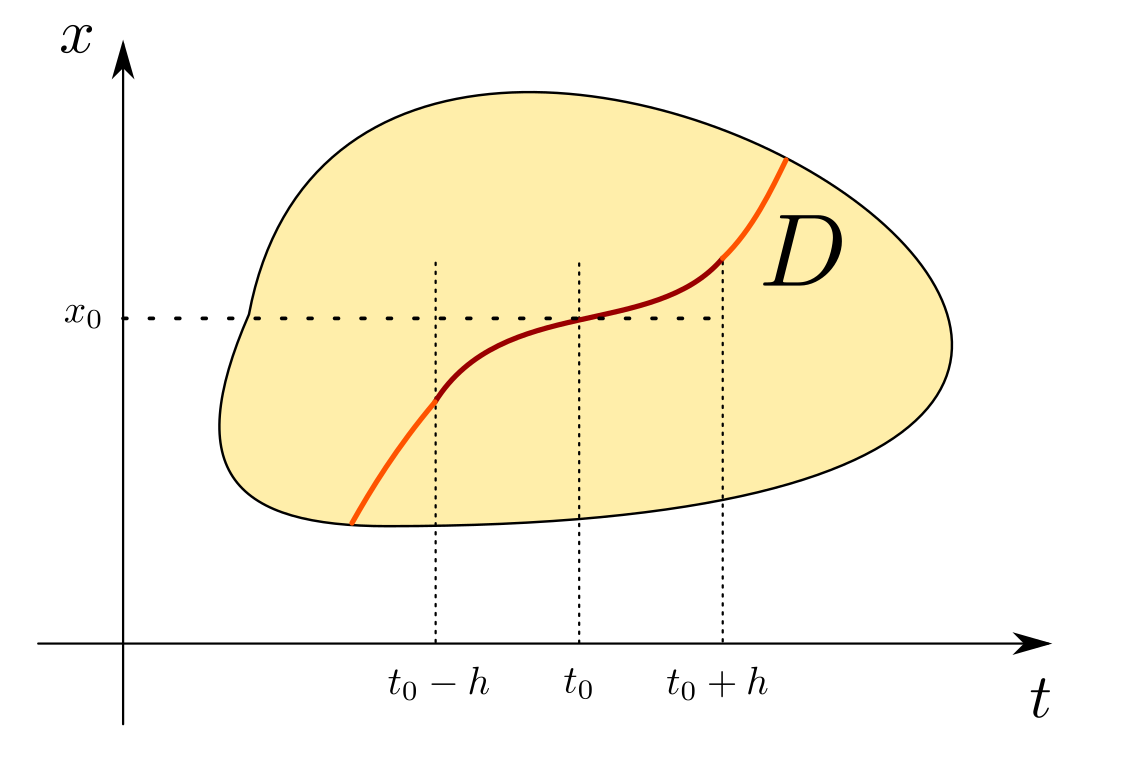
\includegraphics[scale=0.3]{assets/lectures-d0fd0868.png} \end{center}
    Тоді $\exists t^{-} $та  $t^{+} :  t^{-} < t < t^{+}$ такі, що розв'язок задачі Коші з початковою умовою існує на проміжку $ (t^{-}, t^{+})$, причому точки $ (t^-, \overline{x} (t^-)), (t^+, \overline{x} (t^+))$ належать межі області $D$.
\end{boxteo}
\subsection{Основні поняття теорії стійкості.}
Розглянемо систему диф. рівнянь $\overline{x}'(t) = \overline{f} (t, \overline{x})$:
$$f \in   \mathbb{C}(D)\qquad D = [a, +\infty ]  \times G\qquad G \in \mathbb{R}^{n} \qquad  \forall (t_0, \overline{x}^0) \in D  \exists! \text{ розв. З.К. } $$

\bd Розв'язок системи (1) називається стійким за Ляпуновим, якщо:\\
1) $\overline{x} = \overline{\varphi } (t)  \quad \exists$ на $[a, +\infty]$.\\
2) $\forall \varepsilon > 0 \quad \forall t_0 \geq a \quad \exists \delta > 0$, таке, що $ \left|\left| \overline{x}(t_0) - \overline{\varphi}(t_0) \right|\right| < \delta $ справедливо, що $ \left| \left|
\overline{x} (t) - \overline{\varphi} (t)
  \right|  \right|  < \delta  \quad \forall t \geq t_0$.
\ed

\bd
Розв'язок $ \overline{x} = \varphi(t) $ називається асимптотично стійким за лякуновим, якщо:
1. $ \overline{x} = \overline{\varphi} (t)$ - стійкий.\\
2. $\forall t_0 \geq a \quad \exists \delta > 0 \quad \forall \overline{x} (t) $ такого, що $ \left|
\left|  \overline{x} (t_0) - \overline{\varphi} (t_0) \right|
 \right| $ справедливо, що: \\ $  \left|
 \left|  \overline{x} (t) - \overline{\varphi} (t) \right|
  \right| \to 0   $ при $ t \to + \infty$
\ed

\def\vx{\overline{x}}
\def\vphi{\overline{\varphi}}
\def\vf{\overline{f}}

\bd
Роз'язок називається \textbf{нестійким}, якщо він не є стійким.
\ed

\subsection{Прилади дослідження на стійкість за означенням.}

\begin{example}
    Дослідити на стійкість розв'язок З.К.:
$$
\begin{cases}
    x = 1 \\
    x(0) = 0
\end{cases}
$$
1. Знайдемо розв'язок заданої З.К.: $x = 1 \Rightarrow x = t + C$ - заг. розв.\\
Підставимо: $ 0 = 0 + C \Longrightarrow C = 0 \Longrightarrow $ \fbox{ $ \varphi(t) = t $} - будемо досліджувати.
Зазначений розв'язок не має вертикальних асимптот та існує на всьому $\mathbb{R}$.
2. Знайдемо розв'язок довільної З.К. $x(t_0) = x_0$.
$$
x_0 = t_0 + C \Rightarrow C = x_0 - t_0 \Rightarrow x(t) = t + x_0 - t_0
$$
3. Нехай $  \left| x(t_0) - \varphi(t_0) \right|  =  \left| x_0 - t_0 \right| < \delta  $ ;\\
Тоді $ \left| x (t) - \varphi (t) \right|  = \left|  x_0 - t_0 \right| < \varepsilon = \delta $.\\
Таким чином, розв'язок є стійким, але не є асимптотично стійким.

\end{example}

\begin{example}
    Дослідити на стійкість розв'язок З.К.:
    $$
    \begin{cases}
        \dot{x} = 1 + t - x \\
        x(0) = 0
    \end{cases}
    $$
    1. Знайдемо розв'язок даної задачі Коші:
    $$
    \dot{x} = - x + 1 + t = \left| \text{ методом Бернуллі } \right| = t + Ae^{-t}
    $$
    Знайшли загальний розв'язок. Підставимо умову із з. К.: $ A = 0 \Rightarrow \fbox {$\varphi(t) = t$ }$\\
    2. Знайдемо розв'язок довільної З.К.:
    $$
    x(t_0) = x_0 \qquad x_0 = t_0 + Ae^{-t_0} \qquad A = (x_0 - t_0) e^{t_0}
    $$
    $$
    x(t) = t + (x_0 - t_0) e^{t_0 - t} - \text{ загальний розв'язок з. К.}
    $$

    3. Нехай $ \left|  x(t_0) - \varphi(t_0)  \right| = \left| x_0 - t_0 \right|  < \delta $. Розглядаємо: $ \forall t \geq t_0 :$
    $$
    \left| x(t) - \varphi(t) \right| = \left| t + (x_0 - t_0) \cdot e^{ t_0 - t} - t \right| =
     \left| x_0 - t_0 \right|< \delta  \to 0  \quad (t \to + \infty)
    $$
    Отримали, що знайдений розв'язок є асимптотично стійким.
\end{example}
Перейдемо знов до систем диф. рівнянь: $ \vx' = \vf (t, \vx)  \quad (1)$.\\
$\vx = \vphi (t)$ - розв'язок, який ми маємо дослідити на стійкість.\\
Заміна $ \overline{z} (t) = \vx (t)  - \vphi (y) $. Отримаємо систему:
$$ \overline{z}' + \overline{\varphi}'  = \overline{f} (t, \overline{z}+ \overline{\varphi})(t)$$
$$
\overline{f}' (t) = \overline{f} (t, \overline{\varphi})  \Longrightarrow \fbox{ $ \overline{z} ' = \overline{\varphi} (t, \overline{z} + \overline{\varphi} (t)) - \overline{f} ( t, \varphi(t)) $}
$$

Sample



\end{document}
